\documentclass{article}
\usepackage{bm}
\usepackage{amsmath}
\usepackage{amssymb}
\usepackage{graphicx}
\usepackage[colorlinks=true,urlcolor=blue]{hyperref}
\usepackage{geometry}
\geometry{margin=1in}
\usepackage{multicol}
\usepackage{paralist}
\usepackage{todonotes}
\setlength{\marginparwidth}{2.15cm}
\usepackage{booktabs}
\usepackage{enumitem}
\graphicspath{{../}}
\usepackage{setspace}
\doublespacing

\newcommand{\norm}[1]{\left\lVert#1\right\rVert}

\begin{document}

\section*{}
\begin{center}
  \centerline{\textsc{\LARGE Homework 3}}
  \vspace{0.5em}
  \centerline{\textsc{Regression, Gaussian Processes, and Boosting}}
  \vspace{1em}
  \textsc{\large Dana Van Aken} \\
\end{center}

\section*{Problem 1: Gaussian Processes}

\begin{enumerate}[label=(\alph*)]
\setlength\itemsep{1em}

\item A comparison of covariance functions: see figures~\ref{fig:1a1},~\ref{fig:1a2}, and~\ref{fig:1a3}.
\begin{figure}[H]
\centering
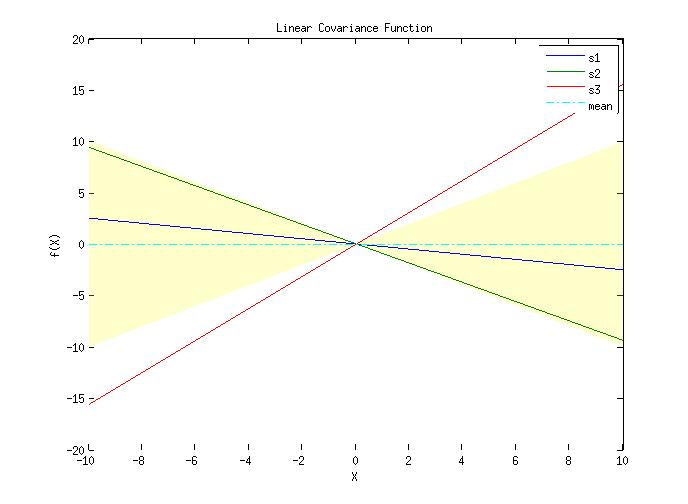
\includegraphics[width=0.8\textwidth]{1_a_1.jpg}
\caption{Linear Covariance Function}
\label{fig:1a1}
\end{figure}
\begin{figure}[H]
\centering
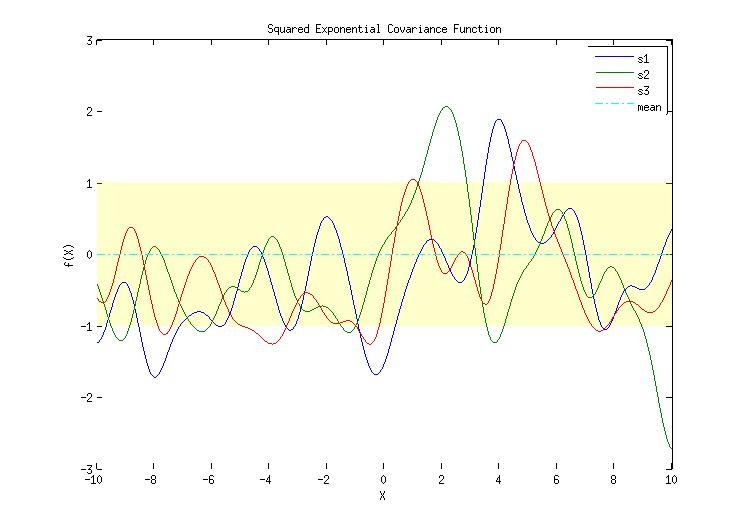
\includegraphics[width=0.8\textwidth]{1_a_2.jpg}
\caption{Square Exponential Covariance Function}
\label{fig:1a2}
\end{figure}
\begin{figure}[H]
\centering
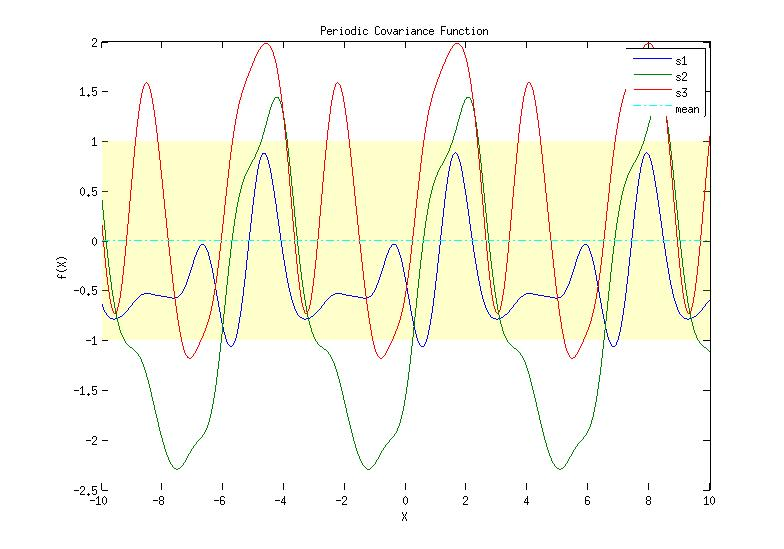
\includegraphics[width=0.8\textwidth]{1_a_3.jpg}
\caption{Periodic Covariance Function}
\label{fig:1a3}
\end{figure}

\item Increasing $\sigma^2$ increases the ``noisyness" of the output points, $y_i$.
Figure~\ref{fig:1b} shows... TODO

\begin{figure}[H]
\centering
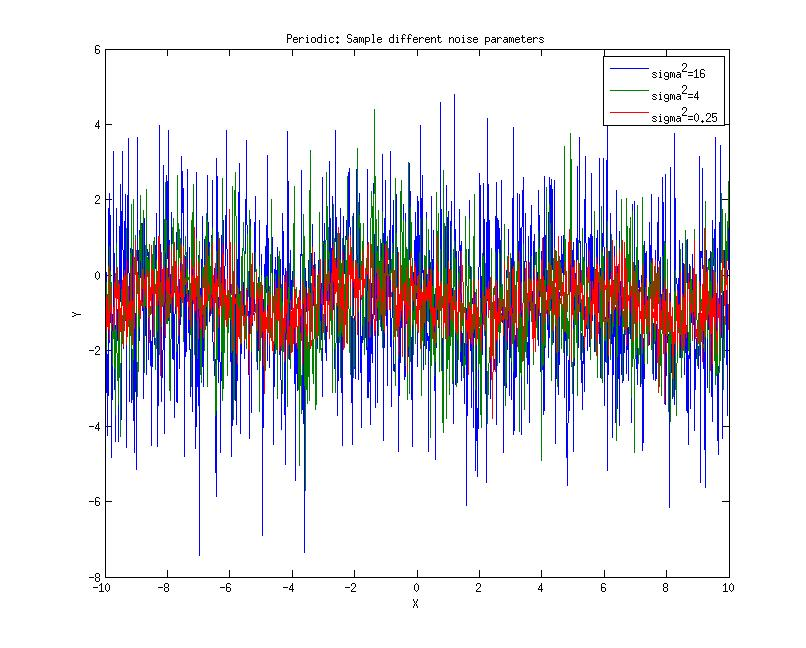
\includegraphics[width=0.8\textwidth]{1_b.jpg}
\caption{Sampling Different Gaussian Noise Parameters Using a Periodic Covariance Function}
\label{fig:1b}
\end{figure}

\item Show $p(x_1|x_2)\propto{}p(x_1,x_2)$ \\
\[
\begin{bmatrix}
  x_1 \\ x_2
\end{bmatrix}
\sim{}N \Bigg(
\begin{bmatrix}
  \mu_1 \\ \mu_2
\end{bmatrix}
\begin{bmatrix}
  \Sigma_{11} & \Sigma{12} \\ \Sigma{21} & \Sigma{22}
\end{bmatrix}
\Bigg)
\]

Let $\Sigma^{-1}=\Lambda^{-1}$ such that
\[
\Sigma^{-1}=
\begin{bmatrix}
  \Sigma_{11} & \Sigma_{12} \\ \Sigma_{21} & \Sigma_{22}
\end{bmatrix}
^{-1}=
\begin{bmatrix}
  \Lambda_{11} & \Lambda_{12} \\ \Lambda_{21} & \Lambda_{22}
\end{bmatrix}
=\Lambda
\]

We can focus on the exponent since we want to find $\mu_{x_1|x_2}$ and $\Sigma_{x_1|x_2}$.

%\begin{equation}
%\begin{align*}
%-\frac{1}{2}(x-\mu)^T\Sigma^{-1}(x-\mu) 
%&=-\frac{1}{2}(x-\mu)^T\Sigma^{-1}(x-\mu) 
%\end{align*}
%\end{equation}

\begin{align*}
exp&=-\frac{1}{2}(x-\mu)^T\Sigma^{-1}(x-\mu) \\
&=-\frac{1}{2}
\begin{bmatrix}
  x_1 - \mu_1 \\ x_2 - \mu_2
\end{bmatrix}
^T
\begin{bmatrix}
  \Sigma_{11} & \Sigma_{12} \\ \Sigma_{21} & \Sigma_{22}
\end{bmatrix}
^{-1}
\begin{bmatrix}
  x_1 - \mu_1 \\ x_2 - \mu_2
\end{bmatrix} \\
&=-\frac{1}{2}
\begin{bmatrix}
  x_1 - \mu_1 \\ x_2 - \mu_2
\end{bmatrix}
^T
\begin{bmatrix}
  \Lambda_{11} & \Lambda_{12} \\ \Lambda_{21} & \Lambda_{22}
\end{bmatrix}
\begin{bmatrix}
  x_1 - \mu_1 \\ x_2 - \mu_2
\end{bmatrix}
\end{align*}

\begin{multline*}
=-\frac{1}{2}(x_1-\mu_1)^T\Lambda_{11}(x_1-\mu_1)
-\frac{1}{2}(x_1-\mu_1)^T\Lambda_{12}(x_2-\mu_2) \\
-\frac{1}{2}(x_2-\mu_2)^T\Lambda_{21}(x_1-\mu_1) 
-\frac{1}{2}(x_2-\mu_2)^T\Lambda_{22}(x_2-\mu_2)
\end{multline*}

We can call the last term, $-\frac{1}{2}(x_2-\mu_2)^T\Lambda_{22}(x_2-\mu_2)$, $C$ since it does not depend on $x_1$ (constant).

\begin{multline*}
=-\frac{1}{2}(x_1-\mu_1)^T\Lambda_{11}(x_1-\mu_1)
-\frac{1}{2}(x_1-\mu_1)^T\Lambda_{12}(x_2-\mu_2)
-\frac{1}{2}(x_2-\mu_2)^T\Lambda_{21}(x_1-\mu_1) 
+C
\end{multline*}

\begin{multline*}
=-\frac{1}{2}x_1^T\Lambda_{11}x_1
+\frac{1}{2}x_1^T\Lambda_{11}\mu_1
+\frac{1}{2}\mu_1^T\Lambda_{11}x_1
-\frac{1}{2}\mu_1^T\Lambda_{11}\mu_1 \\
-\frac{1}{2}x_1^T\Lambda_{12}x_2
+\frac{1}{2}x_1^T\Lambda_{12}\mu_2
+\frac{1}{2}\mu_1^T\Lambda_{12}x_2
-\frac{1}{2}\mu_1^T\Lambda_{12}\mu_2 \\
-\frac{1}{2}x_2^T\Lambda_{21}x_1
+\frac{1}{2}x_2^T\Lambda_{21}\mu_1
+\frac{1}{2}\mu_2^T\Lambda_{21}x_1
-\frac{1}{2}\mu_2^T\Lambda_{21}\mu_1+C
\end{multline*}

Again, include any constants that do not depend on $x_1$ in C.

\begin{multline*}
=-\frac{1}{2}x_1^T\Lambda_{11}x_1
+\frac{1}{2}x_1^T\Lambda_{11}\mu_1
+\frac{1}{2}\mu_1^T\Lambda_{11}x_1
-\frac{1}{2}x_1^T\Lambda_{12}x_2
+\frac{1}{2}x_1^T\Lambda_{12}\mu_2
-\frac{1}{2}x_2^T\Lambda_{21}x_1
+\frac{1}{2}\mu_2^T\Lambda_{21}x_1+C
\end{multline*}

We can use the fact that $\Lambda_{21}=\Lambda_{12}^T$ to reduce the equation.

\begin{equation*}
=-\frac{1}{2}x_1^T\Lambda_{11}x_1
+x_1^T\Lambda_{11}\mu_1
-x_1^T\Lambda_{12}x_2
+x_1^T\Lambda_{12}\mu_2+C
\end{equation*}



\item % (d)

\item A comparison of covariance functions sampled from $p(f(X)|Y_\ast)$: see figures~\ref{fig:1e1},~\ref{fig:1e2}, and~\ref{fig:1e3}.

\begin{figure}[H]
\centering
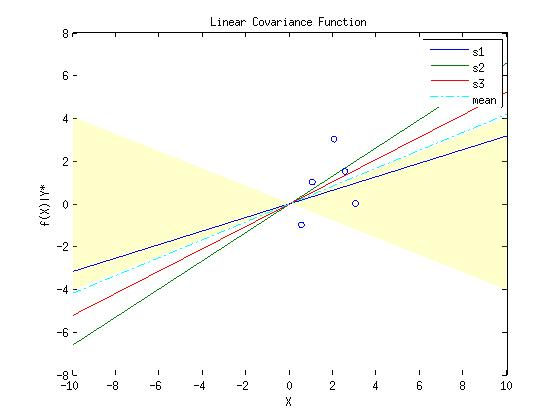
\includegraphics[width=0.8\textwidth]{1_e_1.jpg}
\caption{Linear Covariance Function}
\label{fig:1e1}
\end{figure}
\begin{figure}[H]
\centering
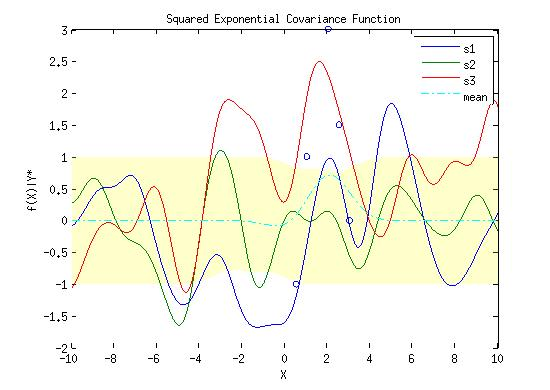
\includegraphics[width=0.8\textwidth]{1_e_2.jpg}
\caption{Square Exponential Covariance Function}
\label{fig:1e2}
\end{figure}
\begin{figure}[H]
\centering
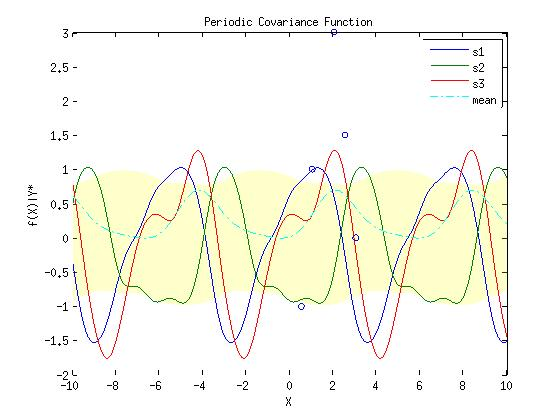
\includegraphics[width=0.8\textwidth]{1_e_3.jpg}
\caption{Periodic Covariance Function}
\label{fig:1e3}
\end{figure}

\item TODO

\begin{figure}[H]
\centering
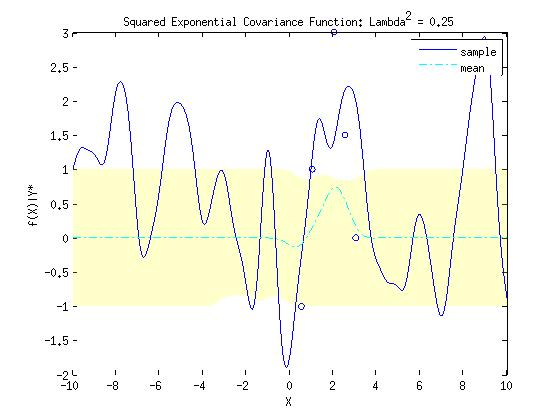
\includegraphics[width=0.8\textwidth]{1_f_1.jpg}
\caption{Sampling Different $\lambda^2$ Parameters Using the Squared Exponential Function}
\label{fig:1f1}
\end{figure}

\begin{figure}[H]
\centering
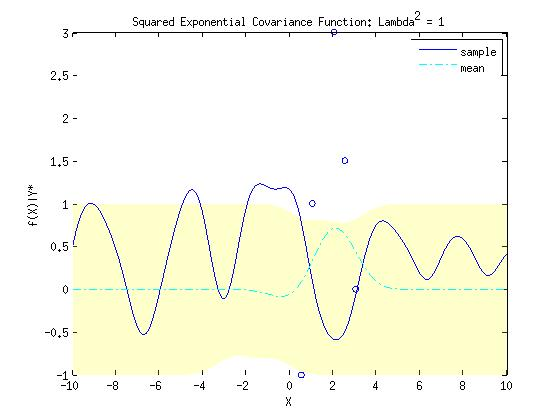
\includegraphics[width=0.8\textwidth]{1_f_2.jpg}
\caption{Sampling Different $\lambda^2$ Parameters Using the Squared Exponential Function}
\label{fig:1f2}
\end{figure}

\begin{figure}[H]
\centering
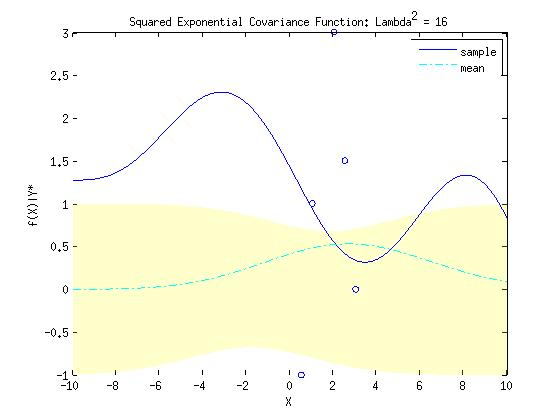
\includegraphics[width=0.8\textwidth]{1_f_3.jpg}
\caption{Sampling Different $\lambda^2$ Parameters Using the Squared Exponential Function}
\label{fig:1f3}
\end{figure}

\end{enumerate}
\end{document}